\documentclass[margin=1cm]{standalone} % fits the pdf to result
\usepackage{tikz} % main package
\usetikzlibrary{decorations.pathreplacing,fit,backgrounds}
\tikzset{
  x = 2cm,
  y = 1.25cm,
  event/.style = { % 'event' node style
    circle,
    draw = #1, % argument = colour
    fill = #1!10, % fade the colour 90% white
    inner sep = 0pt, % no 'padding' b/w text and edge
    minimum width = 8mm, % ensure same size
    minimum height = 8mm,
  },
  distr/.style = { % distribution plot style
    domain = -.5:1.5, % range of x
    samples = 100, % how many samples in the range
    smooth, % smooth the result
    draw = #1,
    fill = #1!10,
  },
  brace/.style = { % using decorations.pathreplacing
    decorate,
    decoration = {brace,amplitude=1ex},
  },
}
\newcommand{\gauss}[3]{ % math of gaussian distribution: #1=x,#2=mu,#3=sd
  1/(#3*sqrt(2*pi))*exp(-0.5*((#1-#2)/#3)^2) }
\begin{document}
  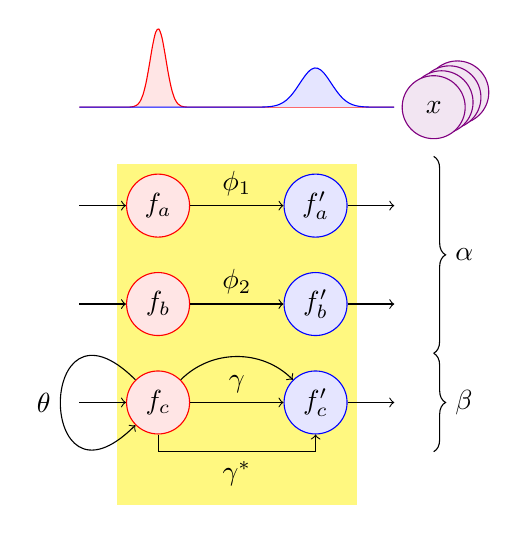
\begin{tikzpicture}
    \foreach \i/\name in {1/a,2/b,3/c}{ % loop through rows
      \def\tmp{\if\i3{\gamma}\else{\phi_\i}\fi} % \if x y compares x==y
      \node[event=red]  (a\i) at (0,-\i) {$f_\name$}; % first event
      \node[event=blue] (b\i) at (1,-\i) {$f'_\name$}; % second event
      \draw[<-] (a\i) -- ++(-.5,0); % in-arrow
      \draw[->] (a\i) -- node[above] {$\tmp$} (b\i); % middle arrow
      \draw[->] (b\i) -- ++(.5,0); % out-arrow
    } % end loop
    \foreach \i in {.15,.10,.05,.00}{ % hack for drawing stacked nodes
      \node[event=red!50!blue] at (1.75+\i,0+\i) {$x$};
    } % end loop
    % more edge options
    \draw (a3) edge[->,out=045,in=135] (b3); % edge: -- with options
    \draw (a3) edge[->,out=135,in=225,looseness=8] node[left]{$\theta$} (a3); % self loop
    \coordinate (x) at (0.5,-3.5); % coord: dummy node
    \draw[->] (a3) |- (x) node[below] (x1) {$\gamma^*$} -| (b3); % -| & |-: square edges
    % braces
    \draw[brace] (1.75,-0.5) -- node[right=1ex]{$\alpha$} (1.75,-2.5); % top brace
    \draw[brace] (1.75,-2.5) -- node[right=1ex]{$\beta$} (1.75,-3.5);  % bottom brace
    \draw[distr=red] plot ({\x},{.1*\gauss{\x}{0}{.05}}); % plot ({x},{y}): first distr
    \draw[distr=blue] plot ({\x},{.1*\gauss{\x}{1}{.1}}); % second distr
    \begin{pgfonlayer}{background} % behind everything
      \node[fill=yellow!50,dotted,fit={(a1)(b3)(x1)}] (box) {}; % auto-fit light yellow box
    \end{pgfonlayer}
  \end{tikzpicture}
\end{document}
